\begin{figure}[htbp]
    \centering
    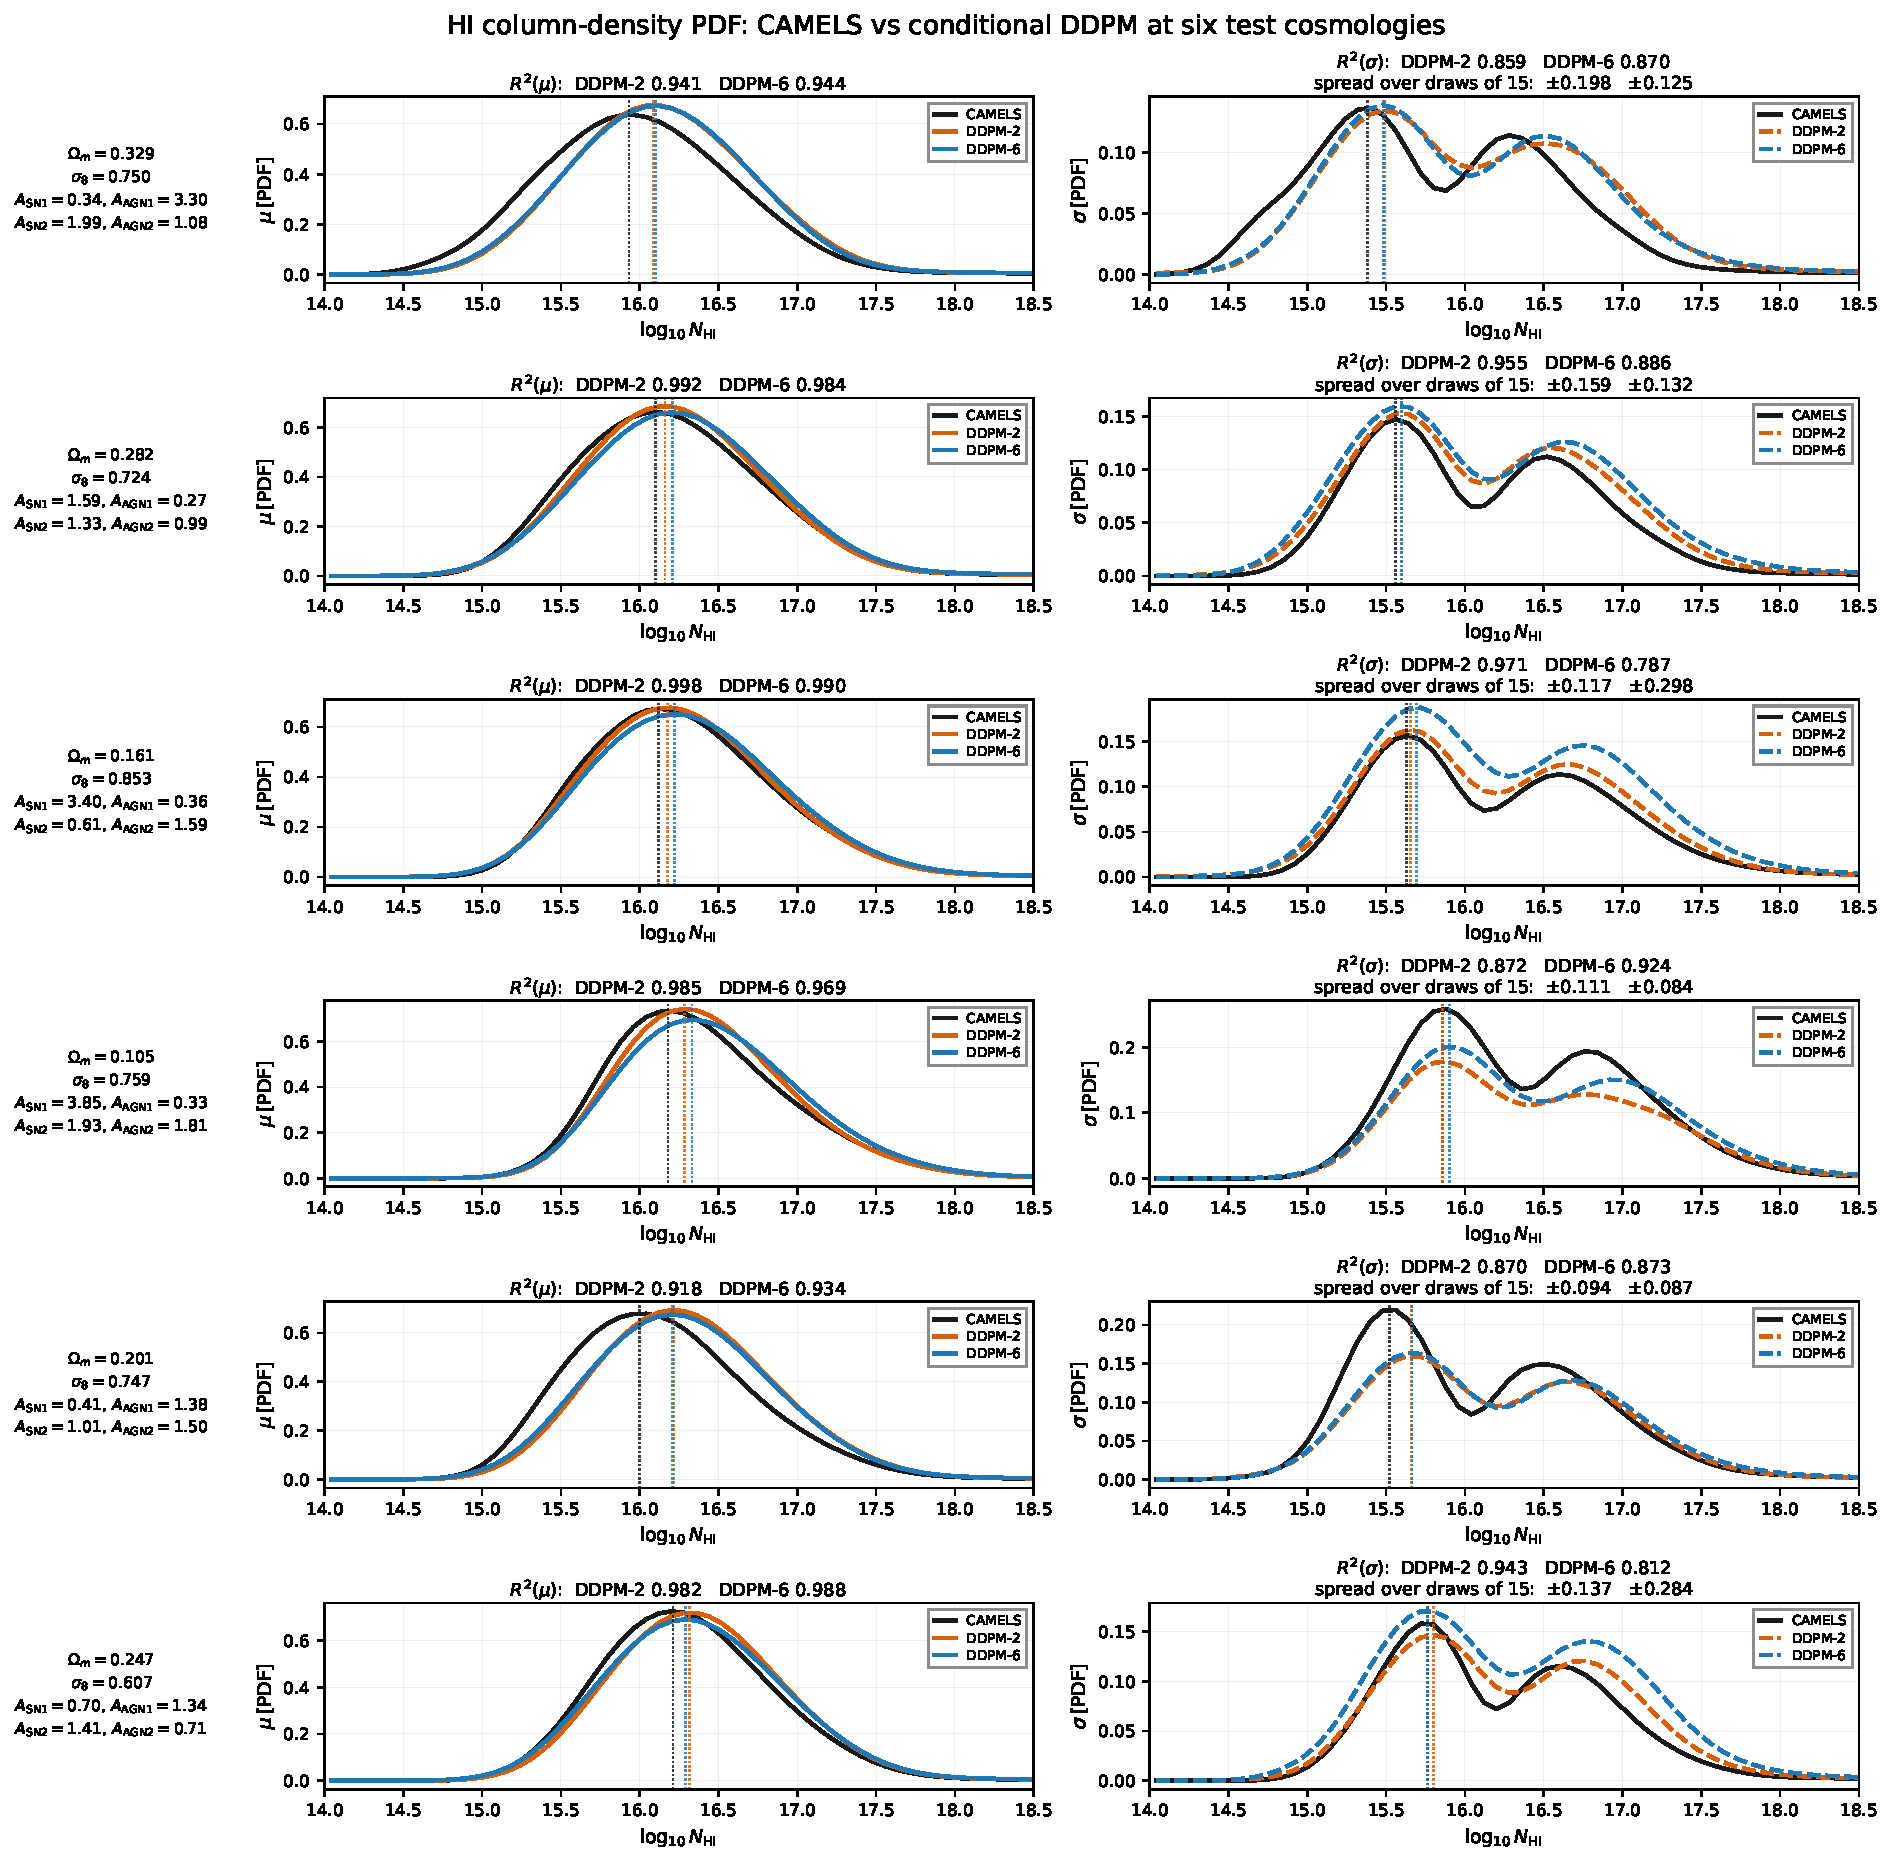
\includegraphics[width=\textwidth]{six_anchor_pdf_labelled_camels_ddpm2_ddpm6.pdf}
    \caption{HI column-density PDF, mean ($\mu$, left) and standard deviation ($\sigma$, right), for CAMELS vs the conditional DDPM-2 and DDPM-6 emulators at six test cosmologies. CAMELS uses the 15 maps the LH set stores at each parameter set (a hard ceiling); 300 maps are generated per emulator. Curves are smoothed for display only, with a 1.5-bin Gaussian applied identically to all three ensembles (quoted $R^2$ and shift statistics use the raw, unsmoothed curves). Dotted verticals mark the measured peak location of each curve, found by parabolic interpolation about the arg-max at sub-bin precision. The horizontal axis is cut at $\log_{10}N_{\rm HI}=18.5$; CAMELS retains 0.9\%--1.9\% of its probability mass above that cut, depending on the anchor.}
    \label{fig:six-anchor-pdf}
\end{figure}
